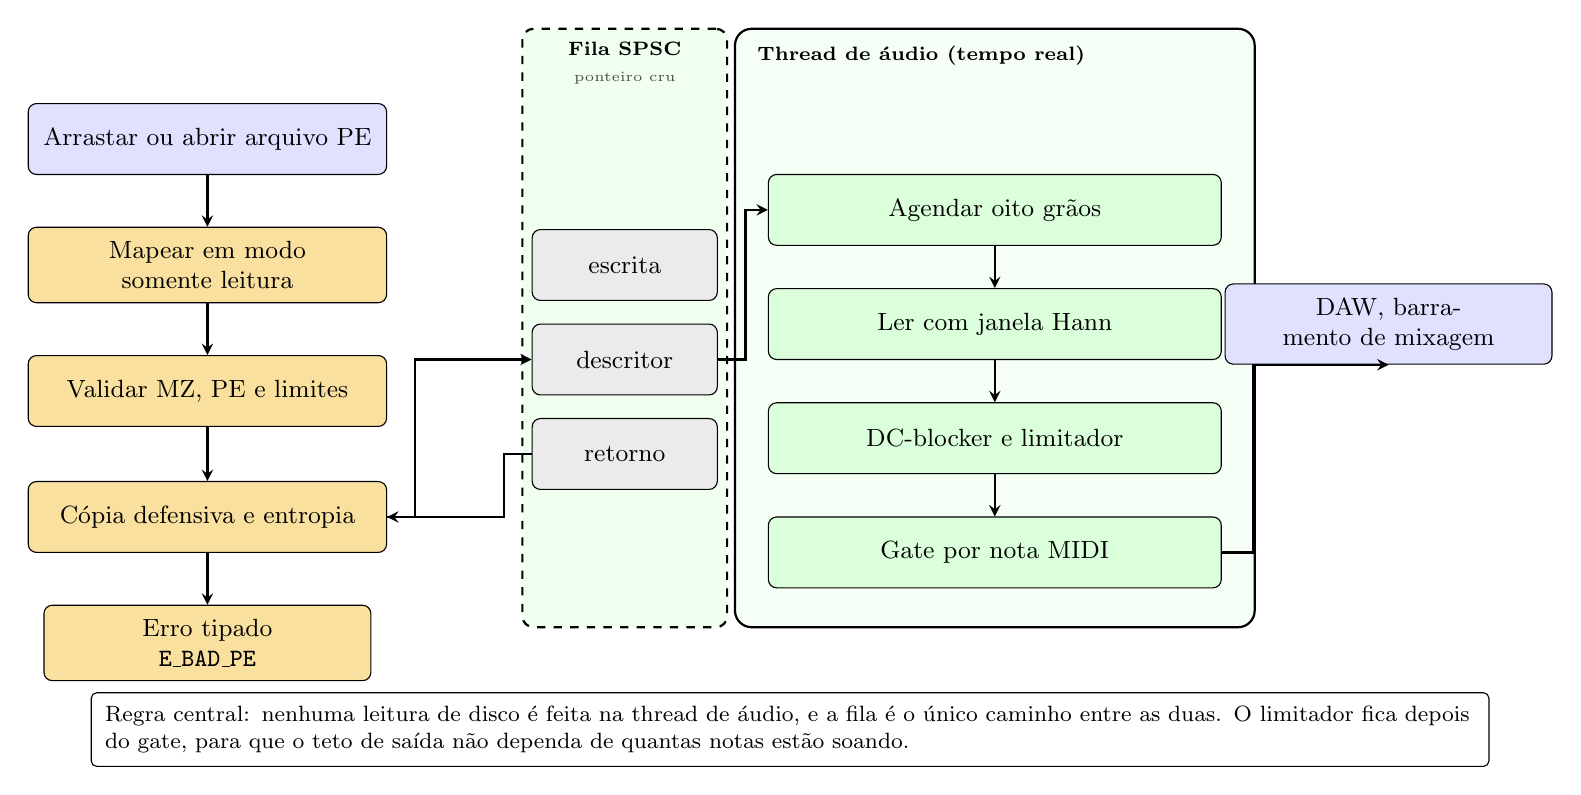
\begin{tikzpicture}
  \definecolor{parserbg}{rgb}{0.98,0.88,0.62}
  \tikzstyle{rt}=[draw, rounded corners=3pt, fill=green!14, minimum height=0.9cm, align=center, font=\small, inner sep=5pt]
  \tikzstyle{ui}=[draw, rounded corners=3pt, fill=blue!12, minimum height=0.9cm, align=center, font=\small, inner sep=5pt]
  \tikzstyle{parse}=[draw, rounded corners=3pt, fill=parserbg, minimum height=0.9cm, align=center, font=\small, inner sep=5pt]
  \tikzstyle{store}=[draw, rounded corners=3pt, fill=gray!16, minimum height=0.9cm, align=center, font=\small, inner sep=5pt]
  \tikzstyle{arr}=[->, >=stealth, thick]
  \tikzstyle{lab}=[font=\tiny, fill=white, inner sep=1.5pt]

  % Coluna da interface e do parser, que nao sao tempo real.
  % As caixas tem 4,2 cm de texto e ficam centradas em x = 0.
  \node[ui, text width=4.2cm] (ui1) at (0,0) {Arrastar ou abrir arquivo PE};
  \node[parse, text width=4.2cm] (p1) at (0,-1.6) {Mapear em modo somente leitura};
  \node[parse, text width=4.2cm] (p2) at (0,-3.2) {Validar MZ, PE e limites};
  \node[parse, text width=4.2cm] (p3) at (0,-4.8) {Cópia defensiva e entropia};
  \node[parse, text width=3.8cm] (perr) at (0,-6.4) {Erro tipado\\\texttt{E\_BAD\_PE}};

  \draw[arr] (ui1) -- (p1);
  \draw[arr] (p1) -- (p2);
  \draw[arr] (p2) -- (p3);
  \draw[arr] (p3) -- (perr);

  % Fila sem trava, a fronteira de tempo real. Comeca depois da coluna de
  % interface: x de 4,0 a 6,6, para nao encostar nas caixas de texto.
  \node[draw, thick, dashed, rounded corners=4pt, fill=green!6, minimum width=2.6cm, minimum height=7.6cm] (frio) at (5.3,-2.4) {};
  \node[font=\scriptsize\bfseries, anchor=north] at (5.3,1.35) {Fila SPSC};
  \node[font=\tiny, anchor=north, text=black!70] at (5.3,0.98) {ponteiro cru};
  \node[store, text width=2.0cm] (f1) at (5.3,-1.6) {escrita};
  \node[store, text width=2.0cm] (f2) at (5.3,-2.8) {descritor};
  \node[store, text width=2.0cm] (f3) at (5.3,-4.0) {retorno};

  \draw[arr] (p3.east) -- ++(0.35,0) |- (f2.west);
  \draw[arr] (f3.west) -- ++(-0.35,0) |- (p3.east);

  % Motor, na thread de audio. Caixas de 5,4 cm centradas em x = 10,0.
  \node[draw, thick, rounded corners=6pt, fill=green!4, minimum width=6.6cm, minimum height=7.6cm] (rtbox) at (10.0,-2.4) {};
  \node[font=\scriptsize\bfseries, anchor=north west] at ([xshift=5pt,yshift=-3pt]rtbox.north west) {Thread de áudio (tempo real)};
  \node[rt, text width=5.4cm] (d1) at (10.0,-0.9) {Agendar oito grãos};
  \node[rt, text width=5.4cm] (d2) at (10.0,-2.35) {Ler com janela Hann};
  \node[rt, text width=5.4cm] (d3) at (10.0,-3.8) {DC-blocker e limitador};
  \node[rt, text width=5.4cm] (d4) at (10.0,-5.25) {Gate por nota MIDI};

  \draw[arr] (f2.east) -- ++(0.35,0) |- (d1.west);
  \draw[arr] (d1) -- (d2);
  \draw[arr] (d2) -- (d3);
  \draw[arr] (d3) -- (d4);

  % Saida para o host
  \node[ui, text width=3.8cm] (daw) at (15.0,-2.35) {DAW, barramento de mixagem};
  \draw[arr] (d4.east) -- ++(0.4,0) |- (daw.south);

  % Legenda de dominio
  \node[draw, fill=white, rounded corners=2pt, align=left, font=\footnotesize, inner sep=5pt, text width=17.4cm] at (7.4,-7.5)
    {Regra central: nenhuma leitura de disco é feita na thread de áudio, e a fila é o único caminho entre as duas. O limitador fica depois do gate, para que o teto de saída não dependa de quantas notas estão soando.};
\end{tikzpicture}
